\documentclass[preprint, 1p]{elsarticle}

\usepackage{lineno,hyperref}
\modulolinenumbers[5]

\journal{the $29^{th}$ ParCFD conference}

%%%%%%%%%%%%%%%%%%%%%%%
%% Elsevier bibliography styles
%%%%%%%%%%%%%%%%%%%%%%%
%% To change the style, put a % in front of the second line of the current style and
%% remove the % from the second line of the style you would like to use.
%%%%%%%%%%%%%%%%%%%%%%%

%% Numbered
%\bibliographystyle{model1-num-names}

%% Numbered without titles
%\bibliographystyle{model1a-num-names}

%% Harvard
%\bibliographystyle{model2-names.bst}\biboptions{authoryear}

%% Vancouver numbered
%\usepackage{numcompress}\bibliographystyle{model3-num-names}

%% Vancouver name/year
%\usepackage{numcompress}\bibliographystyle{model4-names}\biboptions{authoryear}

%% APA style
%\bibliographystyle{model5-names}\biboptions{authoryear}

%% AMA style
%\usepackage{numcompress}\bibliographystyle{model6-num-names}

%% `Elsevier LaTeX' style
\bibliographystyle{elsarticle-num}
%%%%%%%%%%%%%%%%%%%%%%%

\begin{document}

\begin{frontmatter}

\title{Using AmgX to accelerate a PETSc-based Immersed Boundary Method code}

\address[gwu]{Mechanical and Aerospace Engineering, The George Washington University, \\
Washington, DC, 20052, United-States}
\author[gwu]{Olivier Mesnard}
\author[gwu]{Pi-Yueh Chuang}
\author[gwu]{Lorena A. Barba\corref{correspondingauthor}}
\cortext[correspondingauthor]{Corresponding author}
\ead{labarba@gwu.edu}


\begin{abstract}
Our open-source code \texttt{PetIBM}---an immersed boundary method with a fully discrete projection formulation---was written to take advantage of the \texttt{PETSc} library for solving the Poisson system. 
We have now added the capacity to accelerate the time to solution on CUDA-capable GPU devices using the Nvidia library \texttt{AmgX}. 
To provide access to \texttt{AmgX} solvers from a \texttt{PETSc}-based code, we developed a wrapper code that converts the data structures between the two libraries.
This wrapper code could be useful to other \texttt{PETSc} applications that want to use GPUs via \texttt{AmgX}.
Our application of interest is the three-dimensional flow around a  flying-snake,  to reveal the lift-enhancement mechanisms used by this unconventional glider.
We are developing capability to study this problem in Microsoft Azure cloud services.
\end{abstract}

\begin{keyword}
Immersed Boundary Method\sep \texttt{PETSc}\sep \texttt{AmgX} \sep flying snake
\end{keyword}

\end{frontmatter}

\linenumbers

\section{PetIBM and AmgXWrapper}

We have developed \texttt{PetIBM}\footnote{\texttt{PetIBM}: https://github.com/barbagroup/PetIBM}, a code that implements an immersed boundary method (IBM) using the \texttt{PETSc}\footnote{\texttt{PETSc}: https://www.mcs.anl.gov/petsc} library .
The projection method by Taira and Colonius\cite{Taira_Colonius_2007} results in a fully discrete algebraic system that is solved via an approximate block-LU decomposition.
Data structures and routines are provided by the \texttt{PETSc} library, which allowed us to rapidly develop a software that runs on distributed-memory architectures.

As expected with the projection method, the iterative Poisson solver is the bottleneck in our simulations.
This is even worse for the IBM we use where the modified Poisson operator becomes larger and possesses more off-diagonal entries.
To overcome this challenge, we use the Nvidia-library \texttt{AmgX}\footnote{\texttt{AmgX}: https://developer.nvidia.com/amgx} to solve the iterative system on multiple CUDA-capable GPU devices.
We have developed an \texttt{AmgX} wrapper\footnote{\texttt{AmgXWrapper}: https://github.com/barbagroup/AmgXWrapper} that provides the interface with the PETSc library and incorporated it in \texttt{PetIBM}.
Note that this wrapper can used for other \texttt{PETSc} application codes.
Past two-dimensional simulations with \texttt{PetIBM} showed a 21 times application speed-up in runtime from using our \texttt{AmgX} wrapper on one GPU node compared to using \texttt{PETsc} on a CPU node (see Figure \ref{flying_snake_performances}).

The full codes, \texttt{PetIBM} and \texttt{AmgXWrapper}, are open-source, released under MIT license, and version-controlled on GitHub.


\section{Flying snakes to the cloud}

We aim to study the aerodynamics of the \textit{Chrysopelea paradisi}, a species of snake with the amazing capability to glide through the air.
Previous experimental work \cite{Holden_et_al_2014} and two-dimensional simulations \cite{Krishnan_et_al_2014} reported enhanced lift force on a snake gliding at a particular angle of attack of $35^o$.
Using \texttt{PetIBM} and \texttt{AmgXWrapper}, we now intend to understand the three-dimensional wake structures responsible for high gliding performances of the paradise tree snake.

Finally, we decided to use the public cloud Microsoft Azure to run our simulations so that we could compare the performances with our University HPC cluster.

% \begin{figure}[h!]
% \centering
% 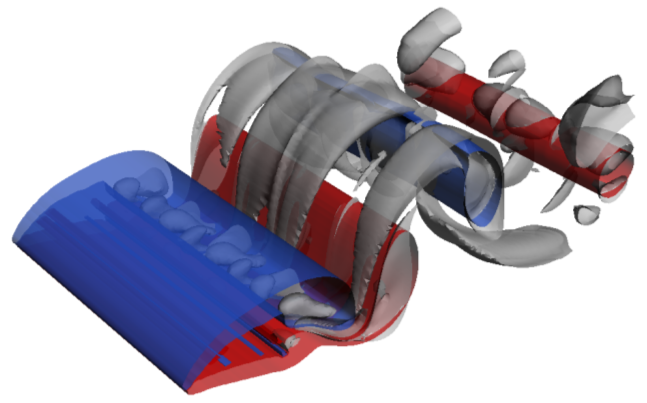
\includegraphics[width=5cm]{images/flying_snake_petibm.png}
% \caption{Vorticity structures in the wake of an infinitely long cylinder with a cross-section of the \textit{Chrysopelea paradisi}.}
% \label{flying_snake_petibm}
% \end{figure}

\begin{figure}[h!]
\centering
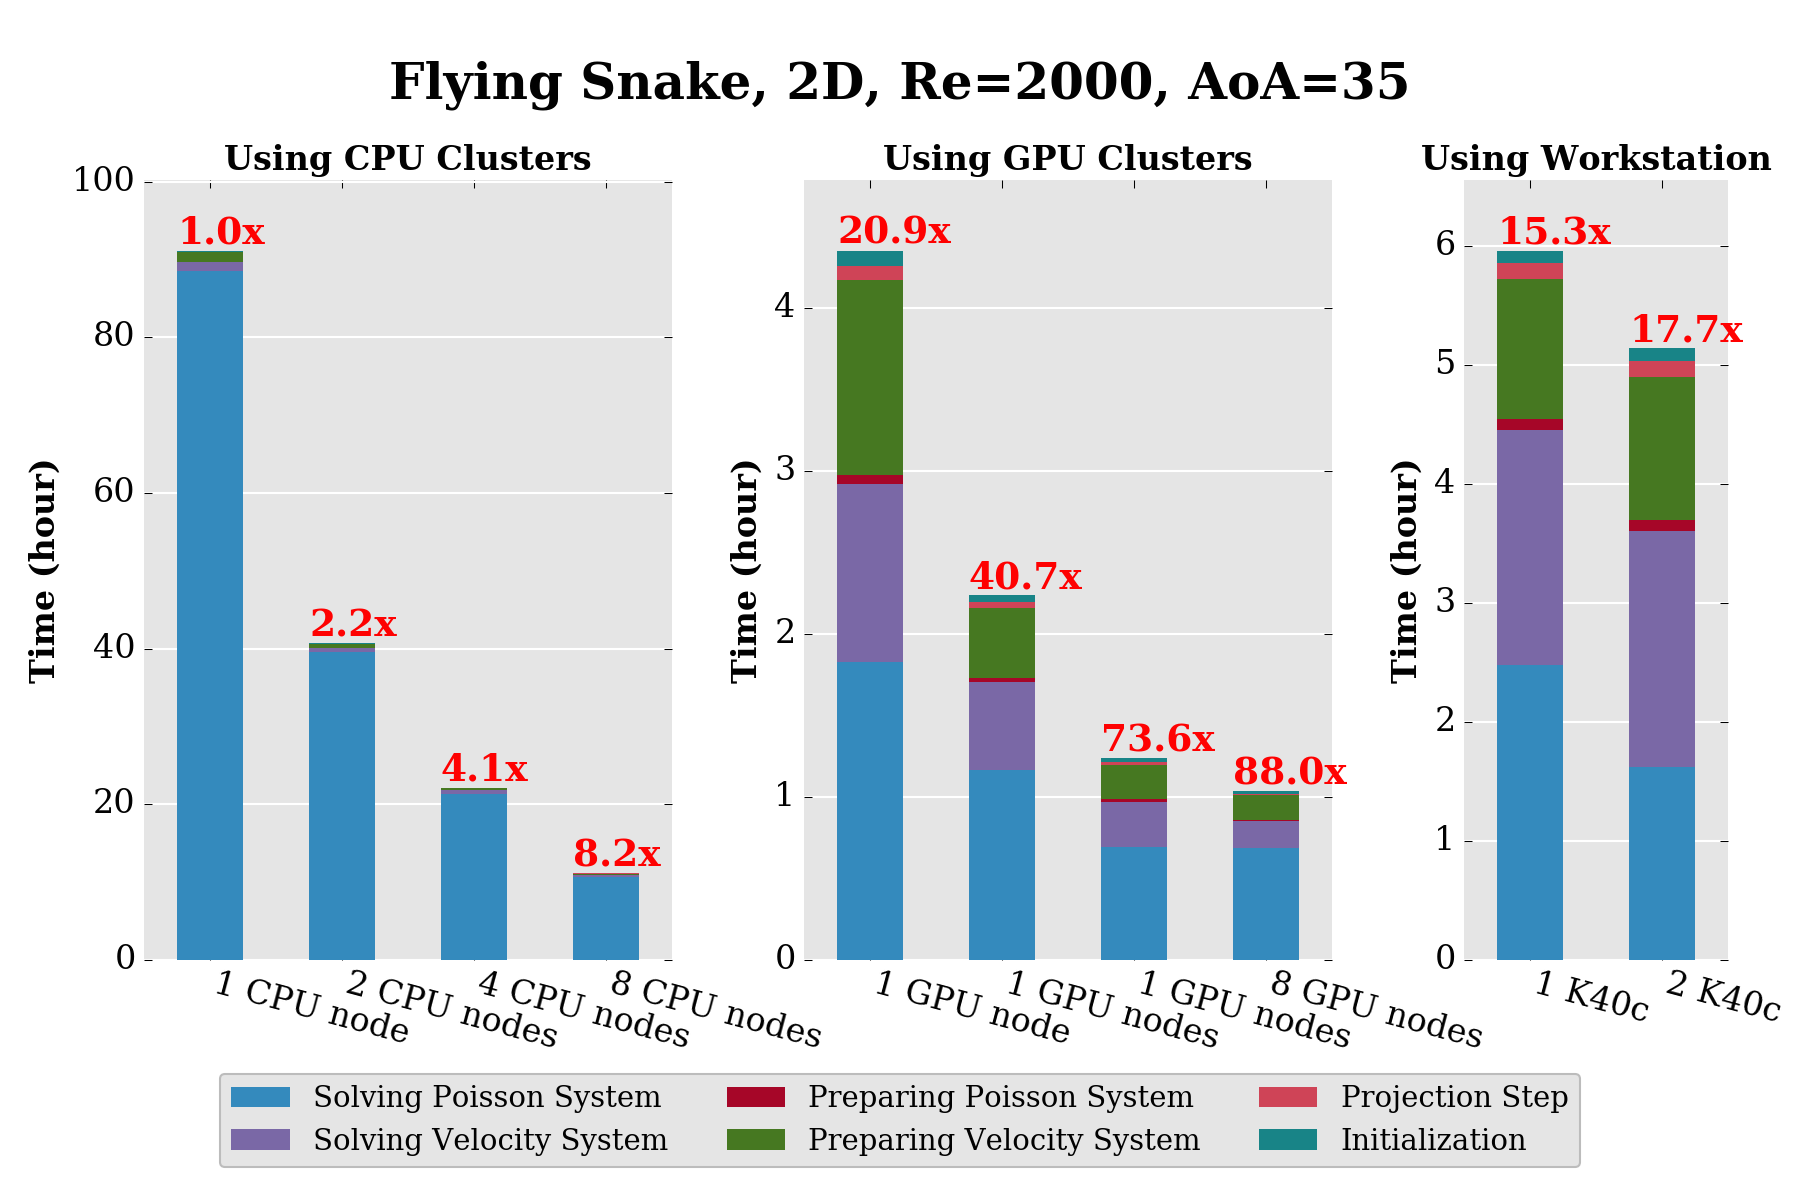
\includegraphics[width=12cm]{images/flying_snake_performances.png}
\caption{Runtimes for the flying-snake case, using \texttt{PetIBM} and \texttt{AmgX}.}
\label{flying_snake_performances}
\end{figure}


\bibliography{references}

\end{document}